% Способ использования БПХ для определения наклона шрифта.

Быстрое преобразование Хафа может быть использовано для определения наклона шрифта. Рассмотрим изображение \ref{img:15_1} с текстом, написанным наклонным шрифтом.
\begin{figure}[!h]
    \centering
    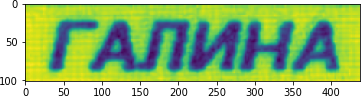
\includegraphics[width=0.7\linewidth]{15_1}
    \caption{Исходное изображение}
    \label{img:15_1}
\end{figure}

Выделим на изображении границы путем вычитания из изображения его дилатации.
\footnote{В данном случае было бы правильнее использовать эрозию, потому что интересующие объекты темнее фона. Однако для этой задачи можно использовать любой метод, потому что нас интересует только наклон выделяющихся прямых, а не точность их позиционирования.}
Результат показан на рисунке \ref{img:15_2}. Также здесь изображение было отражено относительно вертикальной оси, поскольку шрифт, очевидно, наклонен вправо, а стандартная версия быстрого преобразования Хафа работает с прямыми, наклоненными влево с точки стандартной системы координат изображения.
\begin{figure}[!h]
    \centering
    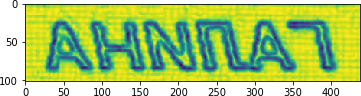
\includegraphics[width=0.7\linewidth]{15_2}
    \caption{Выделенные границы на изображении}
    \label{img:15_2}
\end{figure}

Применим к изображению \ref{img:15_2} БПХ. Результат приведен на изображении \ref{img:15_3}.
\begin{figure}[!h]
    \centering
    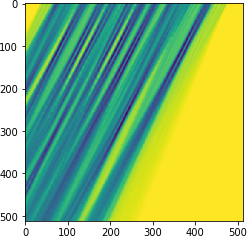
\includegraphics[width=0.35\linewidth]{15_3}
    \caption{Результат применения БПХ к изображению}
    \label{img:15_3}
\end{figure}

В полученном массиве каждая точка описывает сумму значений по некоторой дискретной прямой, причем $i$-я строка соответствует семейству прямых с определенным наклоном $\theta_i = \arctan\left( \frac{n-1}{i} \right)$. Ясно, что среди всех таких семейств то, которое совпадает с наклоном шрифта, будет иметь наибольшую изменчивость: от 0 в промежутках между буквами до высоты строки в случае наложения на <<вертикальный>> элемент буквы. Следовательно, нужно выбрать строку, значения в которой обладают наибольшей дисперсией (или наибольшим стандартным отклонением).
\begin{figure}[!h]
    \centering
    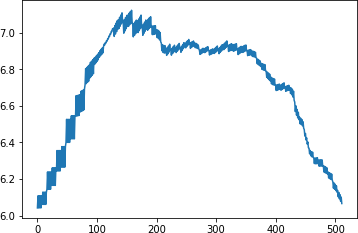
\includegraphics[width=0.5\linewidth]{15_4}
    \caption{График стандартных отклонений строк}
    \label{img:15_4}
\end{figure}

График стандартных отклонений строк приведен на изображении \ref{img:15_4}. В данном случае максимальной дисперсией обладает строка $i=158$, описывающая прямые с наклоном $\theta_{158} = \arctan\left( \frac{511}{158} \right) \approx 73^{\circ}$. Для проверки выведем изображение, наложив поверх него произвольную прямую, обладающую таким наклоном. Как видно по рисунку \ref{img:15_5}, наклон прямой практически совпадает с наклоном шрифта.
\begin{figure}[!h]
    \centering
    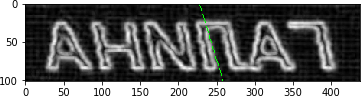
\includegraphics[width=0.5\linewidth]{15_5}
    \caption{Изображение со случайно выбранной прямой из найденного семейства}
    \label{img:15_5}
\end{figure}
